\chapter{Conclusions}

\begin{enumerate}
    \item RQ: Is the TB3 and Husky suited for autonomous driving? 
    
    Both robots are capable of it. The TB3 is limited to even surfaces due to the wheel size and the ball casters. This wheel setup makes the TB3 omnidirectional making it pressies for autonomous driving. 
    The Husky's size make it great for indoor and outdoor use, even though it is capable of autonomous driving the skid turning can be a problem as shown here \ref{Nav2SLAM 2etg}.

    \item RQ: How can the TB3 and the Husky drive autonomously?

    In this thesis this has been accomplished with Xavier connected to TB3/Husky running Ubuntu, ROS2 and Nav2.
    
    \item RQ: How can the TB3 follow the Husky? 

    One method is the logging and replaying the velocity of the Husky, like in the Time Delay \ref{Time delay}. 
    
    \item RQ: How can autonomous platooning be achieved with the TB3 and the Husky? 
    
    Time Delay has been tested as autonomous platooning and the conclusion is it not well suited \ref{HuskyNav2 TBsubpub}. For a safe, stable and smart platooning the Nav2 API method should be used \ref{Further_work_Nav2_API}.
\end{enumerate}



\section{Further work} \label{Further work}

\subsection{Hardware}
\paragraph{The Xaviers} could be switched out with computers using x86 processor for limiting sources of error. 

\paragraph{The Husky} could be switched out with a robot better suited for indoor navigation, the skid turning being the main problem. Moving the LiDAR should also be tested for maximising relevant sensor information. 

\subsection{Improving platooning algorithms}

\paragraph{Nav2 API} \label{Further_work_Nav2_API} was initiated but remained unfinished due to time constraints. This method is based on the Nav2 API and the fact that the TB3 and the Husky have been setup with the ability to drive autonomously independently. For better understanding here is a list of some Nav2 API commands.

\begin{table}[H]
    \centering
    \caption{Some Nav2 API commands \cite{rosnavAPI}.}
    \begin{tabular}{c|c}
        Command             & Description \\ \hline
        setInitialPose()    & Setting initial pose of a robot \\
        goToPose()          & Publishes a Nav2 Goal \\
        goThroughPoses()    & Publishes a list of Nav2 Goals \\
        getPath()           & Receives the complete ongoing path \\
        changeMap()         & Changes current map to chosen one \\
        getFeedback() & Info about the robot running Nav2 like Time stamp, frame\_id and pose\\
    \end{tabular}
    \label{tab:Nav2API}
\end{table}

The idea was both husky and TurtleBot3 run Nav2, a node receives "getFeedback()" from Husky and sends "goToPose()" x distance behind the Husky to the TB3. This task was started on but not finished here is a list with status of the milestones \ref{tab:MilestonesNav2API}.

\begin{table}[H]
    \centering
    \caption{Milestones of Nav2 API.}
    \begin{tabular}{c|c}
        Task                                                        & Status   \\ \hline
        Husky driving autonomously with Nav2                        & Complete \\
        TB3 driving autonomously with Nav2                          & Complete \\
        Control Nav2 with API from python                           & Complete \\
        Control TurtleBot3 simulation with API                      & Complete \\
        Control the Husky with API                                  & Complete \\
        Control the TB3 with API                                    & Complete \\
        TB3 with namespace                                          & Complete \\
        Husky with namespace                                        & Not complete \\
        Running Nav2 on Husky with namespace                        & Not complete \\
        Running Nav2 on TB3 with namespace                          & Not complete \\
        Running Husky and TB3 on same network with independent Nav2 & Not complete\\
        Node receiving position from Husky and sending goal to TB3  & Not complete \\
    \end{tabular}
    \label{tab:MilestonesNav2API}
\end{table}

The main challenge is running two robots with Nav2 simultaneously on the same network. It may be that both robots need two be able to run Nav2 with namespace, but probably just one. Launching two robots may be possible with using the standard launch files from Nav2. It is also possible a custom launch file need to be build using Nav2 nodes like this video \cite{MultiRobotNav2}.
   

\paragraph{AprilTags/ArUco} where researched but not tested. AprilTags and ArUco markers is a system where a camera can get a tf from viewing the tag seen in Figure \ref{fig:apriltags} and demonstrated in Figure \ref{fig:apriltag_principal}. When a tf between TB3 and Husky is acquired this can be used to make a platooning system or improve on an existing one. 

\begin{figure}[H]
  \centering
  \begin{minipage}[b]{0.4\textwidth}
    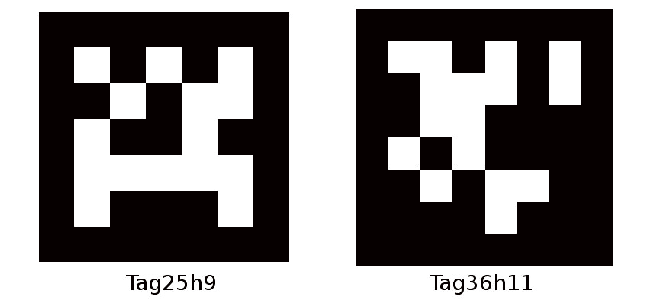
\includegraphics[width=\textwidth]{Figures/images/apriltags.png}
    \caption{Example of two AprilTags}
    \label{fig:apriltags}
  \end{minipage}
  \hfill
  \begin{minipage}[b]{0.4\textwidth}
    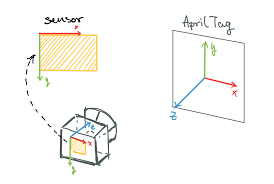
\includegraphics[width=\textwidth]{Figures/images/apriltag_prinsipal.png}
    \caption{Drawing showing the principal of AprilTags}
    \label{fig:apriltag_principal}
  \end{minipage}
\end{figure}

